\documentclass[12pt, letterpaper, twoside]{article}
\usepackage[utf8]{inputenc}
\usepackage{amsmath}
\usepackage{graphicx}
\graphicspath{ {./images/} }


\begin{document}
	
\title{Classification Metrics}
\author{Garima Jain}
\date{\today}
\begin{titlepage}
	\maketitle
\end{titlepage}

\section{Overview}

Formulae discussed in this document are for Binary classification(concerning 2 classes). But these can be extended for the case of Multi-class classification(more than 2 classes)

\section{Precision, Recall and F1 score}

\begin{enumerate}
	\item \textbf{TP}: True Positive(truly/correctly classified as positive)
	\item \textbf{FP}: False Positive(falsely/incorrectly classified as positive)
	\item \textbf{TN}: True Negative(truly/correctly classified as negative)
	\item \textbf{FN}: False Negative(falsely/incorrectly classified as negative)
	\item \textbf{Precision}
	\begin{align}
		Precision = TP / (TP + FP)
	\end{align}
	
	\item \textbf{Recall}(or Sensitivity or True Positive Rate): Represents how many of actual positive samples(TP + FN) have been correctly classified.
	
	\begin{align}
		Recall = TP / (TP + FN)
	\end{align}
	
	\item \textbf{F1 score}: Harmonic mean of Precision and Recall
	\begin{align}
		F1 score = 2 * Precision * Recall / (Precision + Recall)
	\end{align}
	
	\item \textbf{True Negative Rate}(or Specificity): Represents how many of actual negative samples(TN + FP) have been correctly classified.
	
	\begin{align}
		TNR = 1 - FPR =  TN / (TN + FP)
	\end{align}
	
\end{enumerate}

\section{Confusion Matrix}

Matrix of dimension 2x2 representing TP, FN, FP, TN

\section{Receiver Operating Characteristic Curve and AUC(Area under curve)}

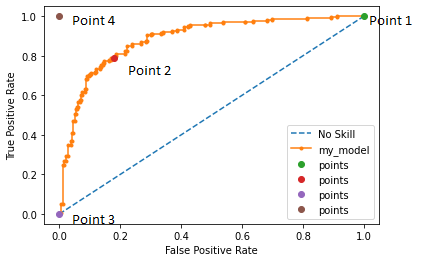
\includegraphics{roc_curve.png}


\end{document}